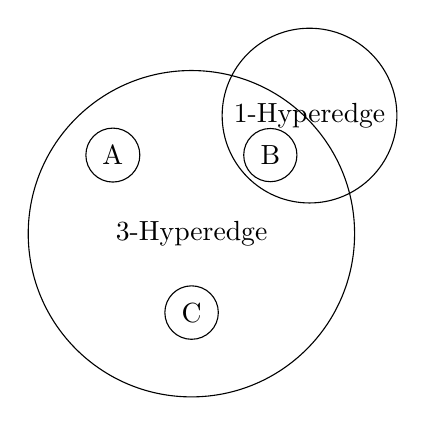
\begin{tikzpicture}
		%\node[draw, align=center] (HEDGE_E) at (-2,2) {
        %    4-Hyperedge
        %};
		%\node[draw, align=center] (HEDGE_D) at (6,0) {
        %    1-Hyperedge
        %};
        %\node[draw, align=center] (HEDGE_A) at (2,0) {
        %    2-Hyperedge
        %};
        %\node[draw, align=center] (HEDGE_B) at (-2,-2) {
        %    0-Hyperedge
        %};
        %\node[draw, align=center] (HEDGE_C) at (6,-2) {
        %    0-Hyperegde
        %};
        %\draw[->, very thick] (HEDGE_A) to (HEDGE_B);
        %\draw[->, very thick] (HEDGE_A) to (HEDGE_C);
        %\draw[->, very thick] (HEDGE_D) to (HEDGE_C);
        %\draw[->, very thick] (HEDGE_E) to (HEDGE_A);
        %\draw[->, very thick] (HEDGE_E) to (HEDGE_B);
        %\draw[->, very thick] (HEDGE_E) to (HEDGE_C);
        %\draw[->, very thick] (HEDGE_E) to (HEDGE_D);
        \node[matrix, circle, draw] (HEDGE_C) at (0,0) {
        	\node[draw,circle] (HEDGE_A) at (-1,0.5) {A};
        	\node[draw,circle] (HEDGE_B) at (1,0.5) {B};
        	\node[] (label) at (0,-0.5) {3-Hyperedge};
        	\node[draw,circle] (HEDGE_F) at (0,-1.5) {C};\\
        };
        \node[draw,circle] (HEDGE_D) at (1.5,1.5) {
        	1-Hyperedge
        };
\end{tikzpicture}